\section{Differentiability}
As we saw when looking at left and right hand derivatives, a derivative will fail to exist when the left and right hand derivatives differ.
However, there are several other cases where a function might not be differentiable at a point.
\begin{enumerate}
	\item \textbf{Corner: } This is the simplest case where both the one sided derivatives exist, are finite, but are different.
		An example would be $f(x)=\abs{x}$ at $x=0$.
	\item \textbf{Cusp: } This is sort of an extreme example of a corner where the one of the one sides derivatives approaches $-\infty$ and the other approaches $\infty$.
		An example would be $f(x)=\sqrt[3]{x^2}$ at $x=0$.
	\item \textbf{Vertical Tangent: } This is where the one sided derivatives exist and agree, but approach $-\infty$ or $\infty$.
		An example would be $f(x)=\sqrt[3]{x}$ at $x = 0$.
	\item \textbf{Discontinuity: } This is where one of the one sided derivatives doesn't exist.
		An example would be the unit step function at $x=0$, which is 1 for $x \geq 0$ and -1 for $x < 0$.
\end{enumerate}

\subsection{Differentiability Implies Local Linearity}
A function is locally linear at a point $a$ when it is differentiable at $a$ and closely resembles its own tangent line at $a$.
Visually, what this means is that as you "zoom in" on a locally linear point, the curve will look more and more like a line.

\begin{figure}[H]
	\label{locally_linear}
	\centering
	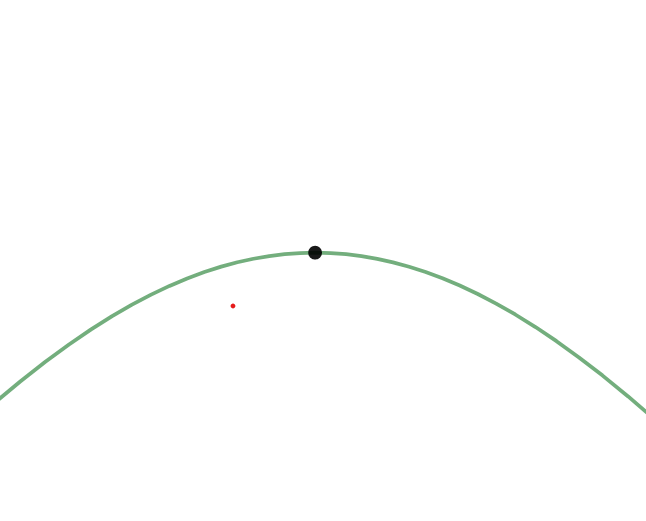
\includegraphics[width = 0.25\textwidth]{./derivatives/cos1.png}
	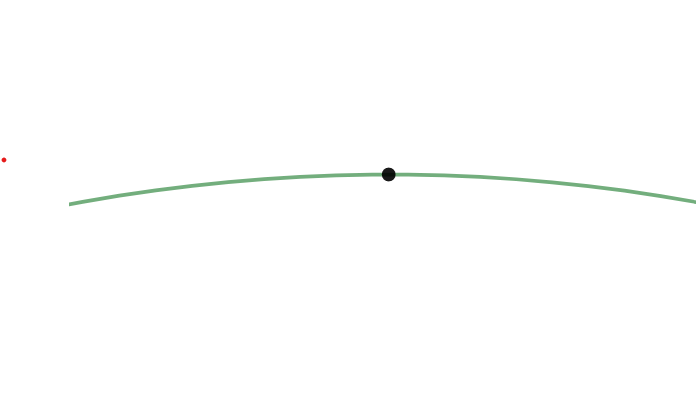
\includegraphics[width = 0.25\textwidth]{./derivatives/cos2.png}
	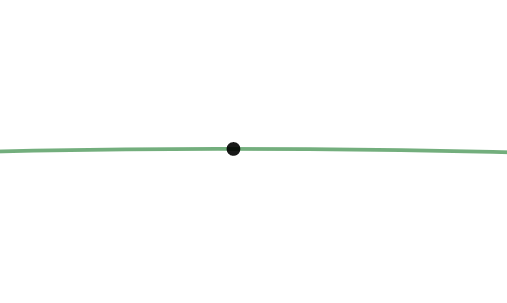
\includegraphics[width = 0.25\textwidth]{./derivatives/cos3.png}
	\caption{\hyperref{}{}{}{Zooming in on a $\cos$ curve}}
\end{figure}

\subsubsection{Numerical Approximation: Symmetric Difference Quotient}
We can use the derivative at a point and a very small value of $h$ to approximate the tangent slope.
However, we can get a better estimate with the same value of $h$ by using the symmetric difference quotient.
\begin{equation*}
	\frac{f(a+h)-f(a-h)}{2h}.
\end{equation*}
\noindent
A calculator might prefer this formula because it tends to give better approximations.

\subsection{Differentiability Implies Continuity}
\begin{theorem}
	If $f^\prime(a)$ exists, then $f$ is continuous at $a$.
\end{theorem}
\noindent
The converse is not necessarily true: a function can be continuous but not differentiable.

\begin{example}
	Determine whether or not the follow function is differentiable at $x=2$.
	\begin{equation*}
		f(x) = \begin{cases}
			x^2 + 1 & x \leq 2 \\
			4x-4 & x > 2
		\end{cases}.
	\end{equation*}
\end{example}
Looking at the graph of this function, we see there is a jump discontinuity at $x=2$.
If the function was differentiable at $x=2$, it would be continuous at $x=2$.
Since it is not continuous at $x=2$, it must not be differentiable at $x=2$.
